\documentclass[border=8pt]{standalone}
\usepackage[T1]{fontenc}
\usepackage{mathptmx}
\usepackage{tikz}
\usetikzlibrary{arrows.meta,positioning,fit,calc,shapes.geometric,shapes.misc,shapes.multipart,backgrounds}
\tikzset{
  arr/.style={-{Stealth[length=2.4mm,width=1.8mm]},line width=0.6pt},
  box/.style={draw,line width=0.6pt,align=center,rounded corners=2pt},
}

\begin{document}
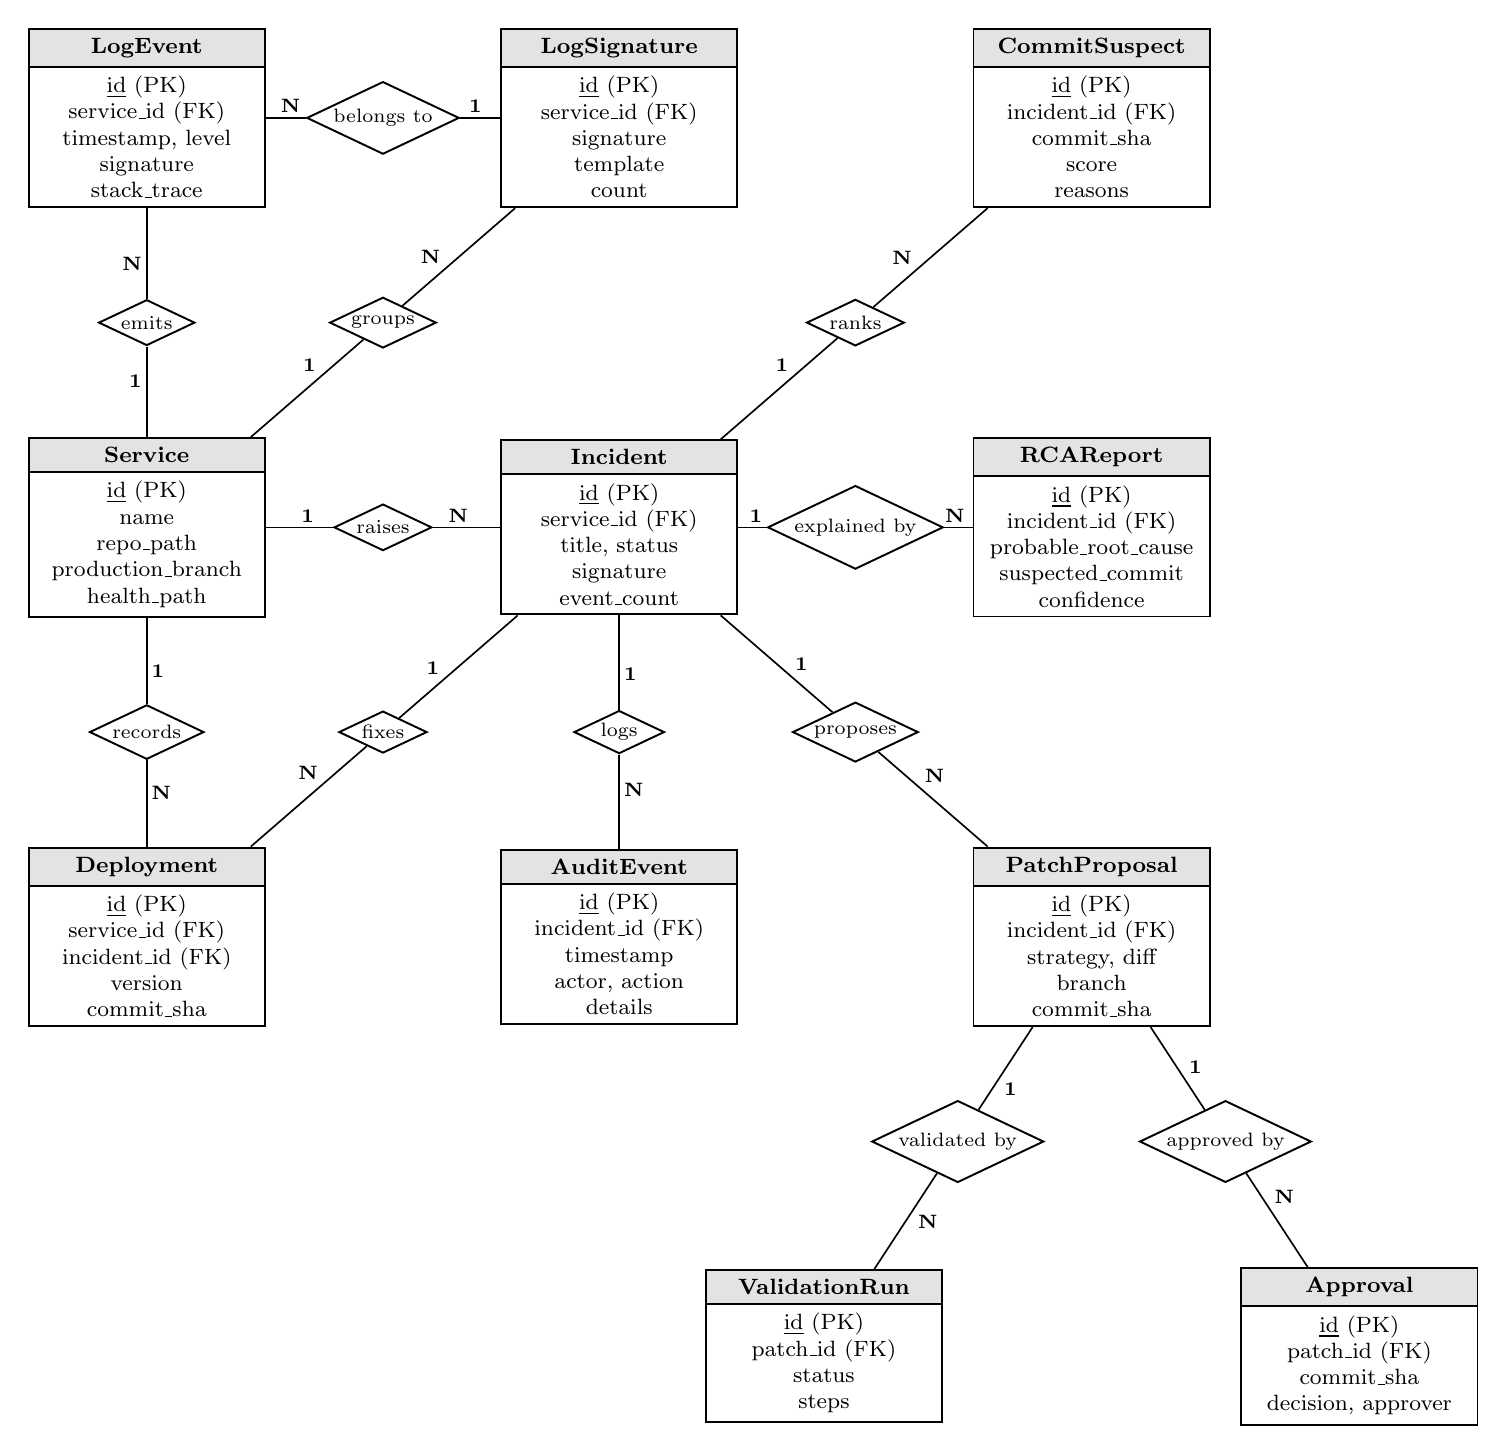
\begin{tikzpicture}[font=\footnotesize,
 ent/.style={draw, line width=0.7pt, rectangle split, rectangle split parts=2, rectangle split part fill={gray!22,white}, minimum width=3.0cm, align=center, inner sep=3pt},
 rel/.style={draw, diamond, aspect=2.1, line width=0.7pt, inner sep=1pt, font=\scriptsize, align=center, fill=white},
 card/.style={font=\scriptsize\bfseries, inner sep=1.5pt}]
\node[ent] (service) at (-6,0) {\textbf{Service}\nodepart{two}\underline{id} (PK)\\ name\\ repo\_path\\ production\_branch\\ health\_path};
\node[ent] (logevent) at (-6,5.2) {\textbf{LogEvent}\nodepart{two}\underline{id} (PK)\\ service\_id (FK)\\ timestamp, level\\ signature\\ stack\_trace};
\node[ent] (logsig) at (0,5.2) {\textbf{LogSignature}\nodepart{two}\underline{id} (PK)\\ service\_id (FK)\\ signature\\ template\\ count};
\node[ent] (deploy) at (-6,-5.2) {\textbf{Deployment}\nodepart{two}\underline{id} (PK)\\ service\_id (FK)\\ incident\_id (FK)\\ version\\ commit\_sha};
\node[ent] (incident) at (0,0) {\textbf{Incident}\nodepart{two}\underline{id} (PK)\\ service\_id (FK)\\ title, status\\ signature\\ event\_count};
\node[ent] (audit) at (0,-5.2) {\textbf{AuditEvent}\nodepart{two}\underline{id} (PK)\\ incident\_id (FK)\\ timestamp\\ actor, action\\ details};
\node[ent] (suspect) at (6,5.2) {\textbf{CommitSuspect}\nodepart{two}\underline{id} (PK)\\ incident\_id (FK)\\ commit\_sha\\ score\\ reasons};
\node[ent] (rca) at (6,0) {\textbf{RCAReport}\nodepart{two}\underline{id} (PK)\\ incident\_id (FK)\\ probable\_root\_cause\\ suspected\_commit\\ confidence};
\node[ent] (patch) at (6,-5.2) {\textbf{PatchProposal}\nodepart{two}\underline{id} (PK)\\ incident\_id (FK)\\ strategy, diff\\ branch\\ commit\_sha};
\node[ent] (valrun) at (2.6,-10.4) {\textbf{ValidationRun}\nodepart{two}\underline{id} (PK)\\ patch\_id (FK)\\ status\\ steps};
\node[ent] (approval) at (9.4,-10.4) {\textbf{Approval}\nodepart{two}\underline{id} (PK)\\ patch\_id (FK)\\ commit\_sha\\ decision, approver};
\node[rel] (r0) at (-6,2.6) {emits};
\draw[line width=0.6pt] (service) -- node[card, pos=0.62, auto] {1} (r0) -- node[card, pos=0.38, auto] {N} (logevent);
\node[rel] (r1) at (-3,5.2) {belongs to};
\draw[line width=0.6pt] (logevent) -- node[card, pos=0.62, auto] {N} (r1) -- node[card, pos=0.38, auto] {1} (logsig);
\node[rel] (r2) at (-3,2.6) {groups};
\draw[line width=0.6pt] (service) -- node[card, pos=0.62, auto] {1} (r2) -- node[card, pos=0.38, auto] {N} (logsig);
\node[rel] (r3) at (-3,0) {raises};
\draw[line width=0.6pt] (service) -- node[card, pos=0.62, auto] {1} (r3) -- node[card, pos=0.38, auto] {N} (incident);
\node[rel] (r4) at (-6,-2.6) {records};
\draw[line width=0.6pt] (service) -- node[card, pos=0.62, auto] {1} (r4) -- node[card, pos=0.38, auto] {N} (deploy);
\node[rel] (r5) at (-3,-2.6) {fixes};
\draw[line width=0.6pt] (deploy) -- node[card, pos=0.62, auto] {N} (r5) -- node[card, pos=0.38, auto] {1} (incident);
\node[rel] (r6) at (0,-2.6) {logs};
\draw[line width=0.6pt] (incident) -- node[card, pos=0.62, auto] {1} (r6) -- node[card, pos=0.38, auto] {N} (audit);
\node[rel] (r7) at (3,2.6) {ranks};
\draw[line width=0.6pt] (incident) -- node[card, pos=0.62, auto] {1} (r7) -- node[card, pos=0.38, auto] {N} (suspect);
\node[rel] (r8) at (3,0) {explained by};
\draw[line width=0.6pt] (incident) -- node[card, pos=0.62, auto] {1} (r8) -- node[card, pos=0.38, auto] {N} (rca);
\node[rel] (r9) at (3,-2.6) {proposes};
\draw[line width=0.6pt] (incident) -- node[card, pos=0.62, auto] {1} (r9) -- node[card, pos=0.38, auto] {N} (patch);
\node[rel] (r10) at (4.3,-7.8) {validated by};
\draw[line width=0.6pt] (patch) -- node[card, pos=0.62, auto] {1} (r10) -- node[card, pos=0.38, auto] {N} (valrun);
\node[rel] (r11) at (7.7,-7.8) {approved by};
\draw[line width=0.6pt] (patch) -- node[card, pos=0.62, auto] {1} (r11) -- node[card, pos=0.38, auto] {N} (approval);
\end{tikzpicture}
\end{document}